\section{Micro-P4 \;($\mu$P4)}
Re-configurable targets process packets using multiple type of processing blocks and P4 provides multiple sub-languages following heterogenous abstract machines to program the blocks.
The presence of heterogeneous abstract machines and device-specific constructs is the
primary reason for lack of mechanisms for modularity and code reuse.
Because, it is not possible to define interface to reuse code modules when caller and callee modules can have incompatible abstract machines.


$\mu$P4 comprise of an architecture, $\mu$SA, and a compiler, $\mu$P4C for a logical target device. 
$\mu$SA simplifies abstract machine for P4 data plane programs by exposing minimal number of programmable blocks required to implement.
It provides abstraction by defining logical externs that allows programmers to express packet processing logic that is outside the scope of current P4 and relies on fixed-function blocks in real targets.
$\mu$SA defines generic interfaces to enable easy code reuse of fine-grained packet-processing functions and build new functions.
We associate runtime behavior with the generic interface as described in Section \ref{subsection:packet-processing-using-mp4}. 
$\mu$P4C allows programmer to express \emph{sequential} and \emph{parallel} packet processing of multiple fine-grained functions using instances of their types.
$\mu$P4C enables composition of packet-processing functions using P4 language itself, unlike Hyper4 and P4Visor which rely on different configuration languages.
$\mu$P4C translates simplified abstract machine and its logical externs into real target-specific heterogeneous packet-processing blocks, features and constraints.


\subsection{Packet Processing using $\mu$P4}
\label{subsection:packet-processing-using-mp4}
We model every packet-processing function as a black-box micro-switch that processes packet byte-stream, intrinsic metadata and user-defined parameters as shown in Figure \ref{fig:package-runtime-behavior}.
The black-box model hides implementation details (headers types, user-defined metadata, programmable blocks etc.,) of micro-switches.
To realise this model, $\mu$SA defines multiple packet-processing pipelines and each pipeline is associated with one or more generic interface types.
Each generic interface exposes a set of programmable blocks to implement and allows programmers to specify type parameters for runtime arguments.
Programmers can implement the interfaces and define new \emph{package} types.
In control blocks of $\mu$SA pipelines, the package types can be instantiated and invoked by supplying arguments for the defined runtime parameters. 
\begin{figure}[!h]
    \centering
    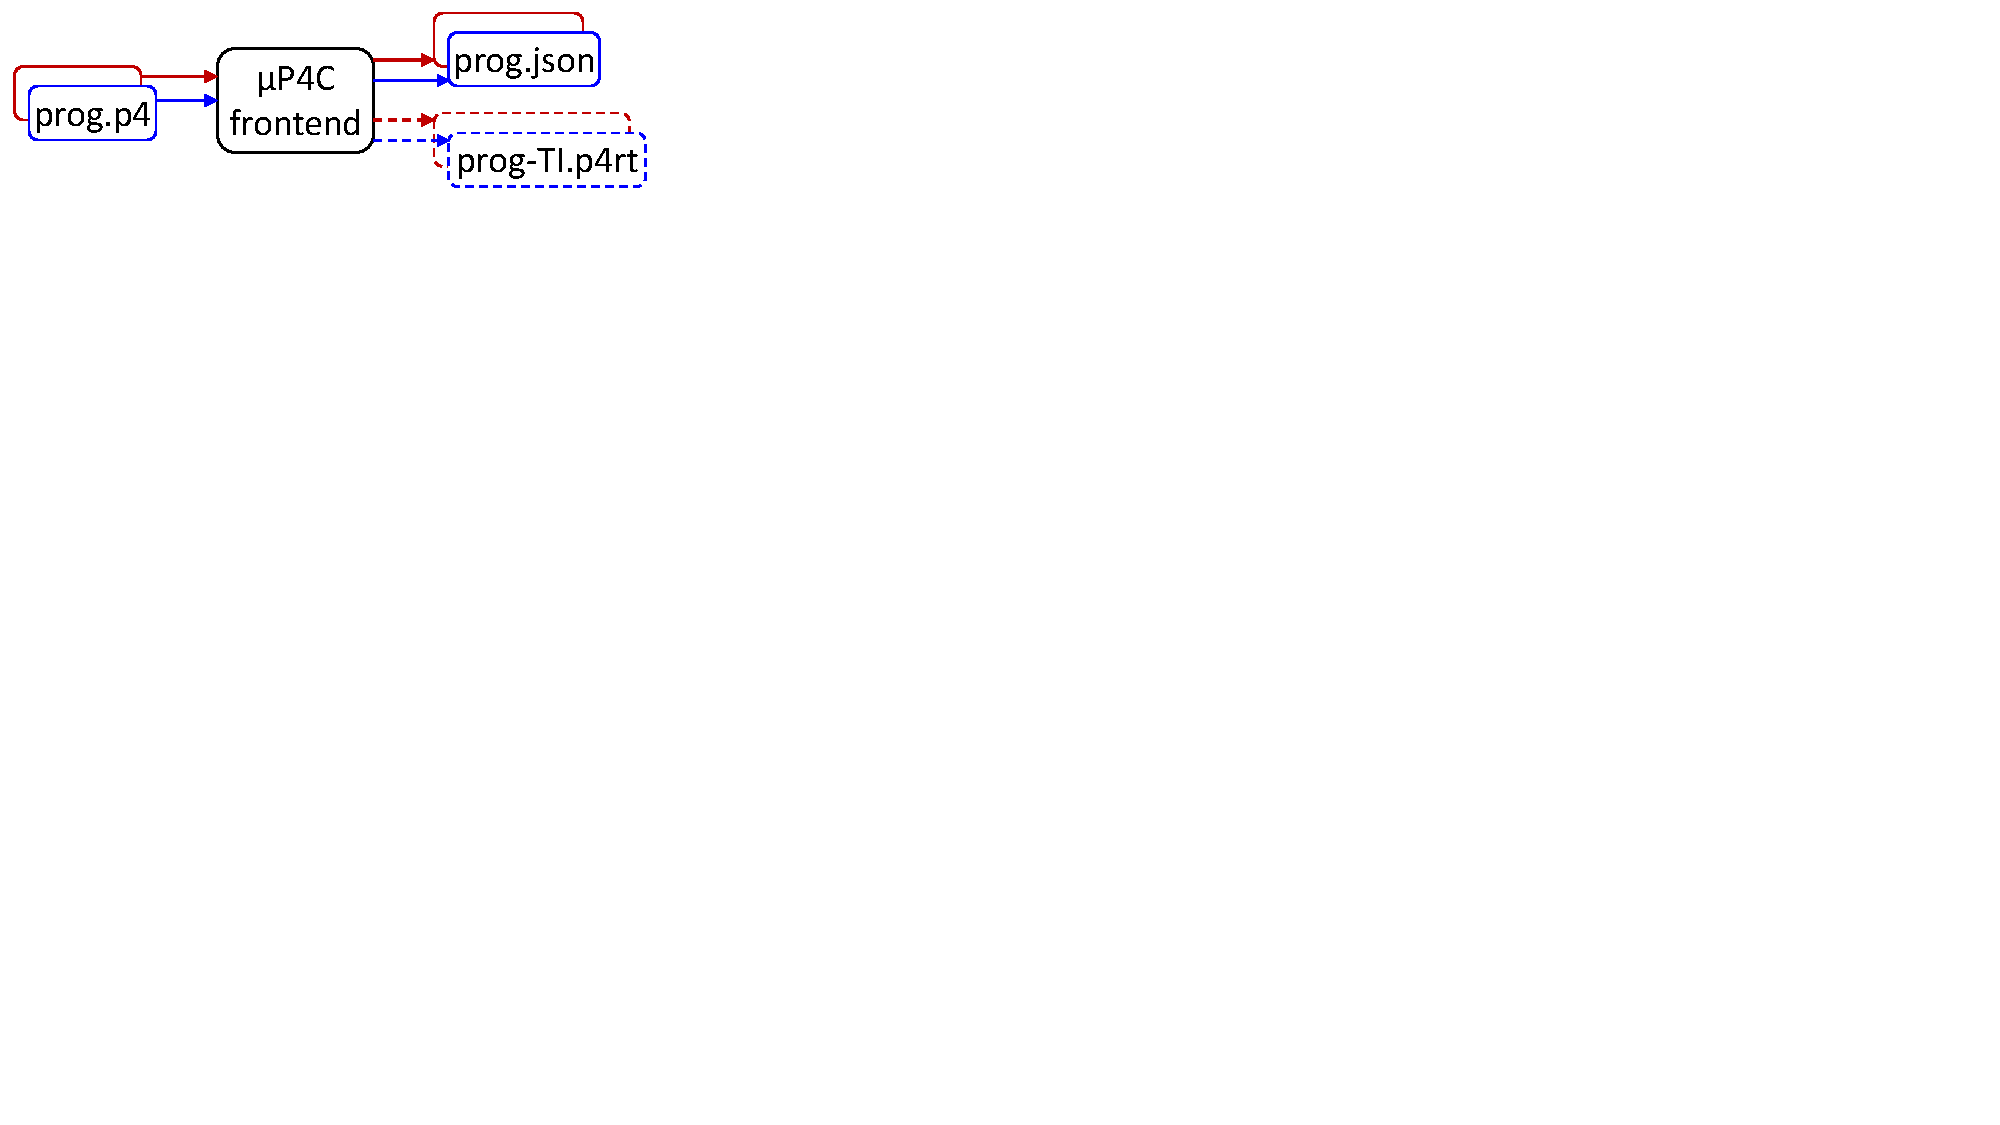
\includegraphics[trim=300 300 0 0, clip,scale=0.2]{mp4c-frontend}
    \caption{Micro P4 Package Runtime Behavior}
    \label{fig:package-runtime-behavior}
\end{figure}


\subsubsection{Sequential Processing}
In sequential processing, packets modified by one function are processed by another functions.
$\mu$P4 facilitates sequential processing by treating user-defined packages types similar to control types in existing P4 language.
Programmers can invoke micro-switch modules using its package interface in body of control blocks other micro-switch modules.


\subsubsection{Parallel Processing}
In parallel processing, multiple micro-switch process a copy 

\subsection{Compiling $\mu$P4 programs}

% Third, we develop compiler mechanisms to have uniform abstract-machine for programmable blocks.
% Finally, we translate our unified abstract machine and logical externs into real target-specific heterogeneous packet-processing blocks, features and constraints.


% In this section, we present a system, $\mu$P4, comprising of an architecture, $\mu$SA for a logical target device and a compiler, $\mu$P4C, to compile $\mu$SA-specific code to real target-specific code.

% In section \ref{section:micros-awitch-architecture}, we explain the design of Micro Switch Architecture for a logical target that reduces number of programmable blocks and introduces logical externs to minimize heterogeneity in abstract model of P4 programs.







% What do we need to provide interface to code modules?
% 
% We need runtime behaviour with package. 
% packet, sm, es, inargs, inout args -> package -> packet, sm, es, out args, inout args
% P4 extended to 
% allow Define new Package types
% runtime behavior with package types
% 
% MicroP4 defines package interfaces.
% 
% 
% MicroP4 captures intrinsic metadata dependency of real targets using logical extern (egress\_spec)
% 
% MicroP4 defines common abstractions for target specific operations that can not be expressed in P4
% e.g., multicast




\begin{figure}[!h]
    \begin{subfigure}{\linewidth}
        \centering
        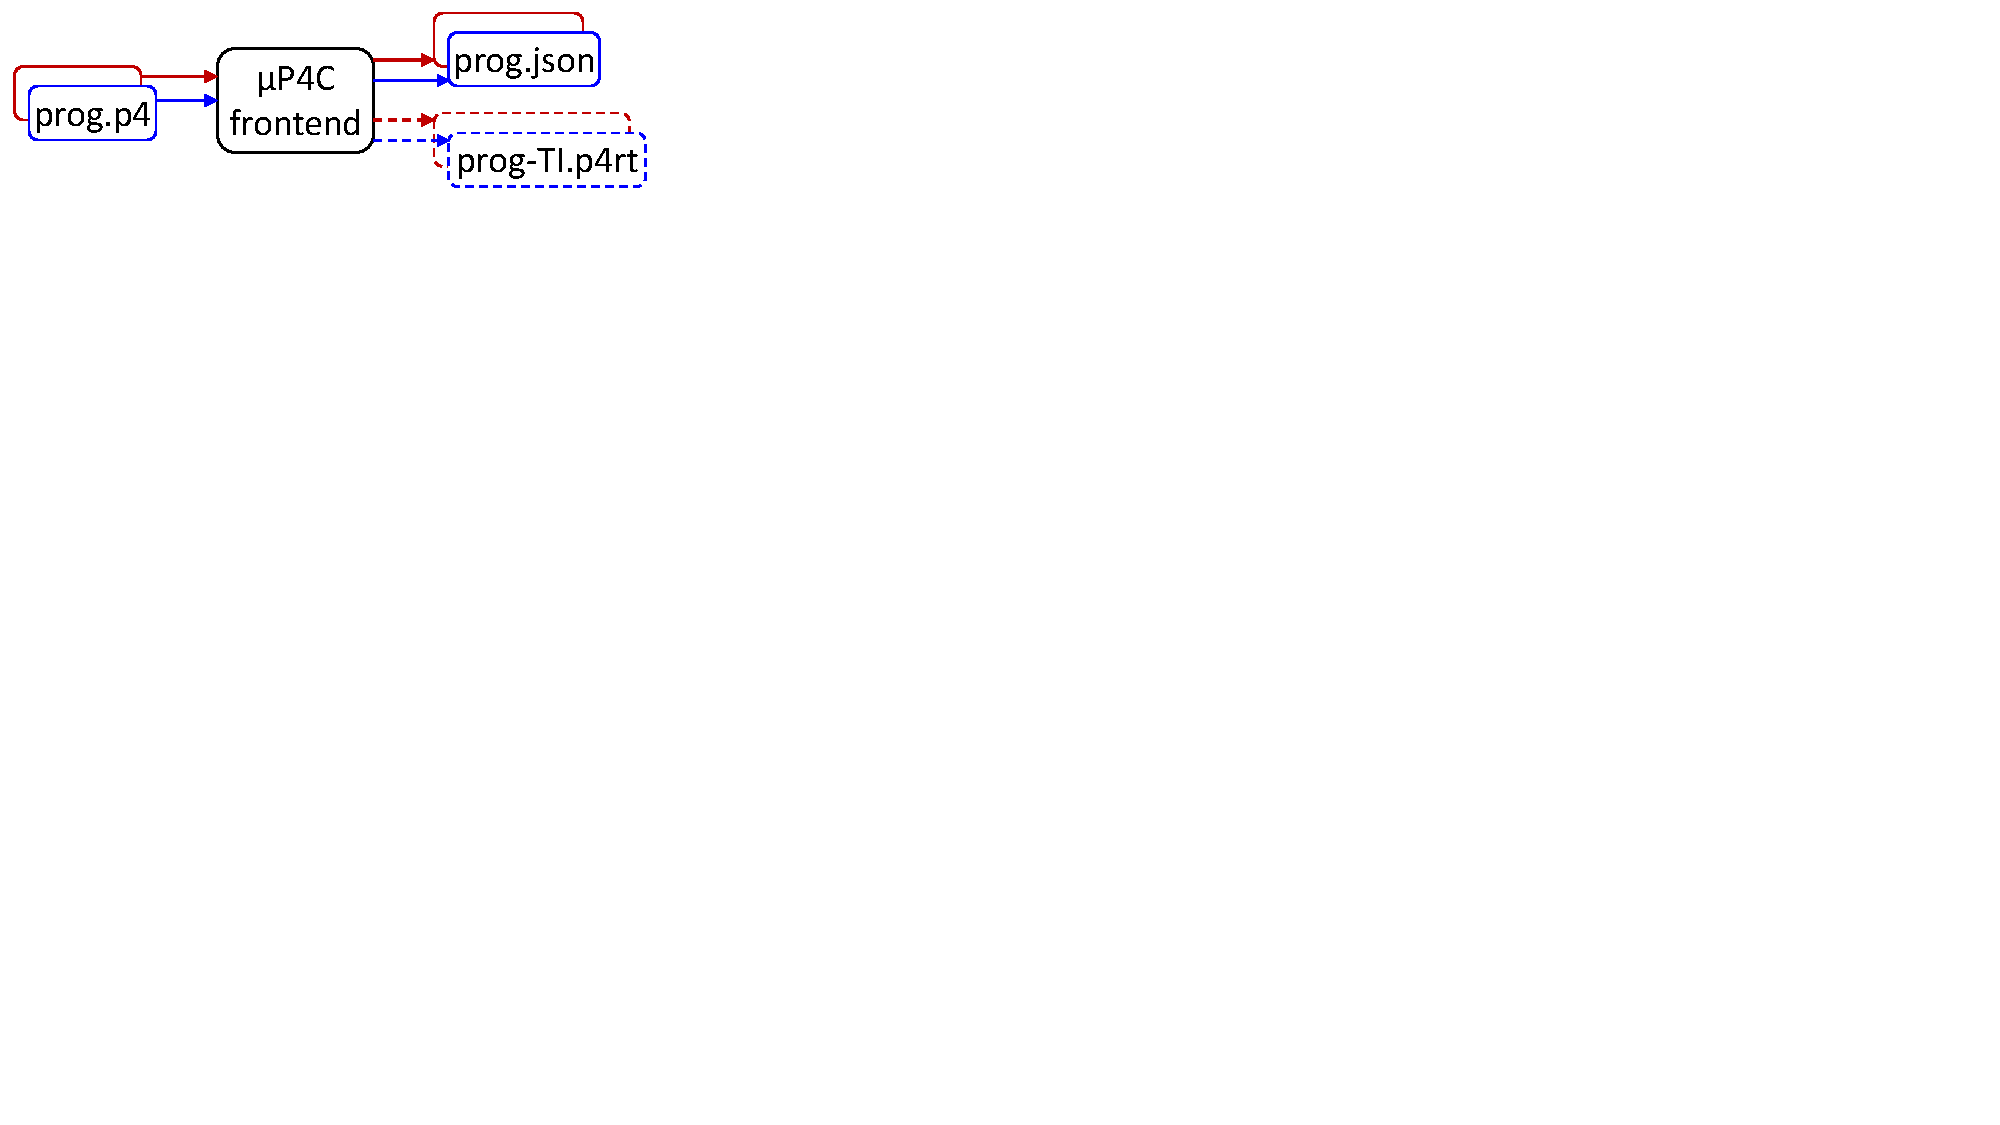
\includegraphics[trim=0 435 665 0, clip,scale=0.55]{mp4c-frontend}
        \caption{Library Program Compilation}
        \label{subfig:compiling-modules}
    \end{subfigure}
    \begin{subfigure}{\linewidth}
        \centering
        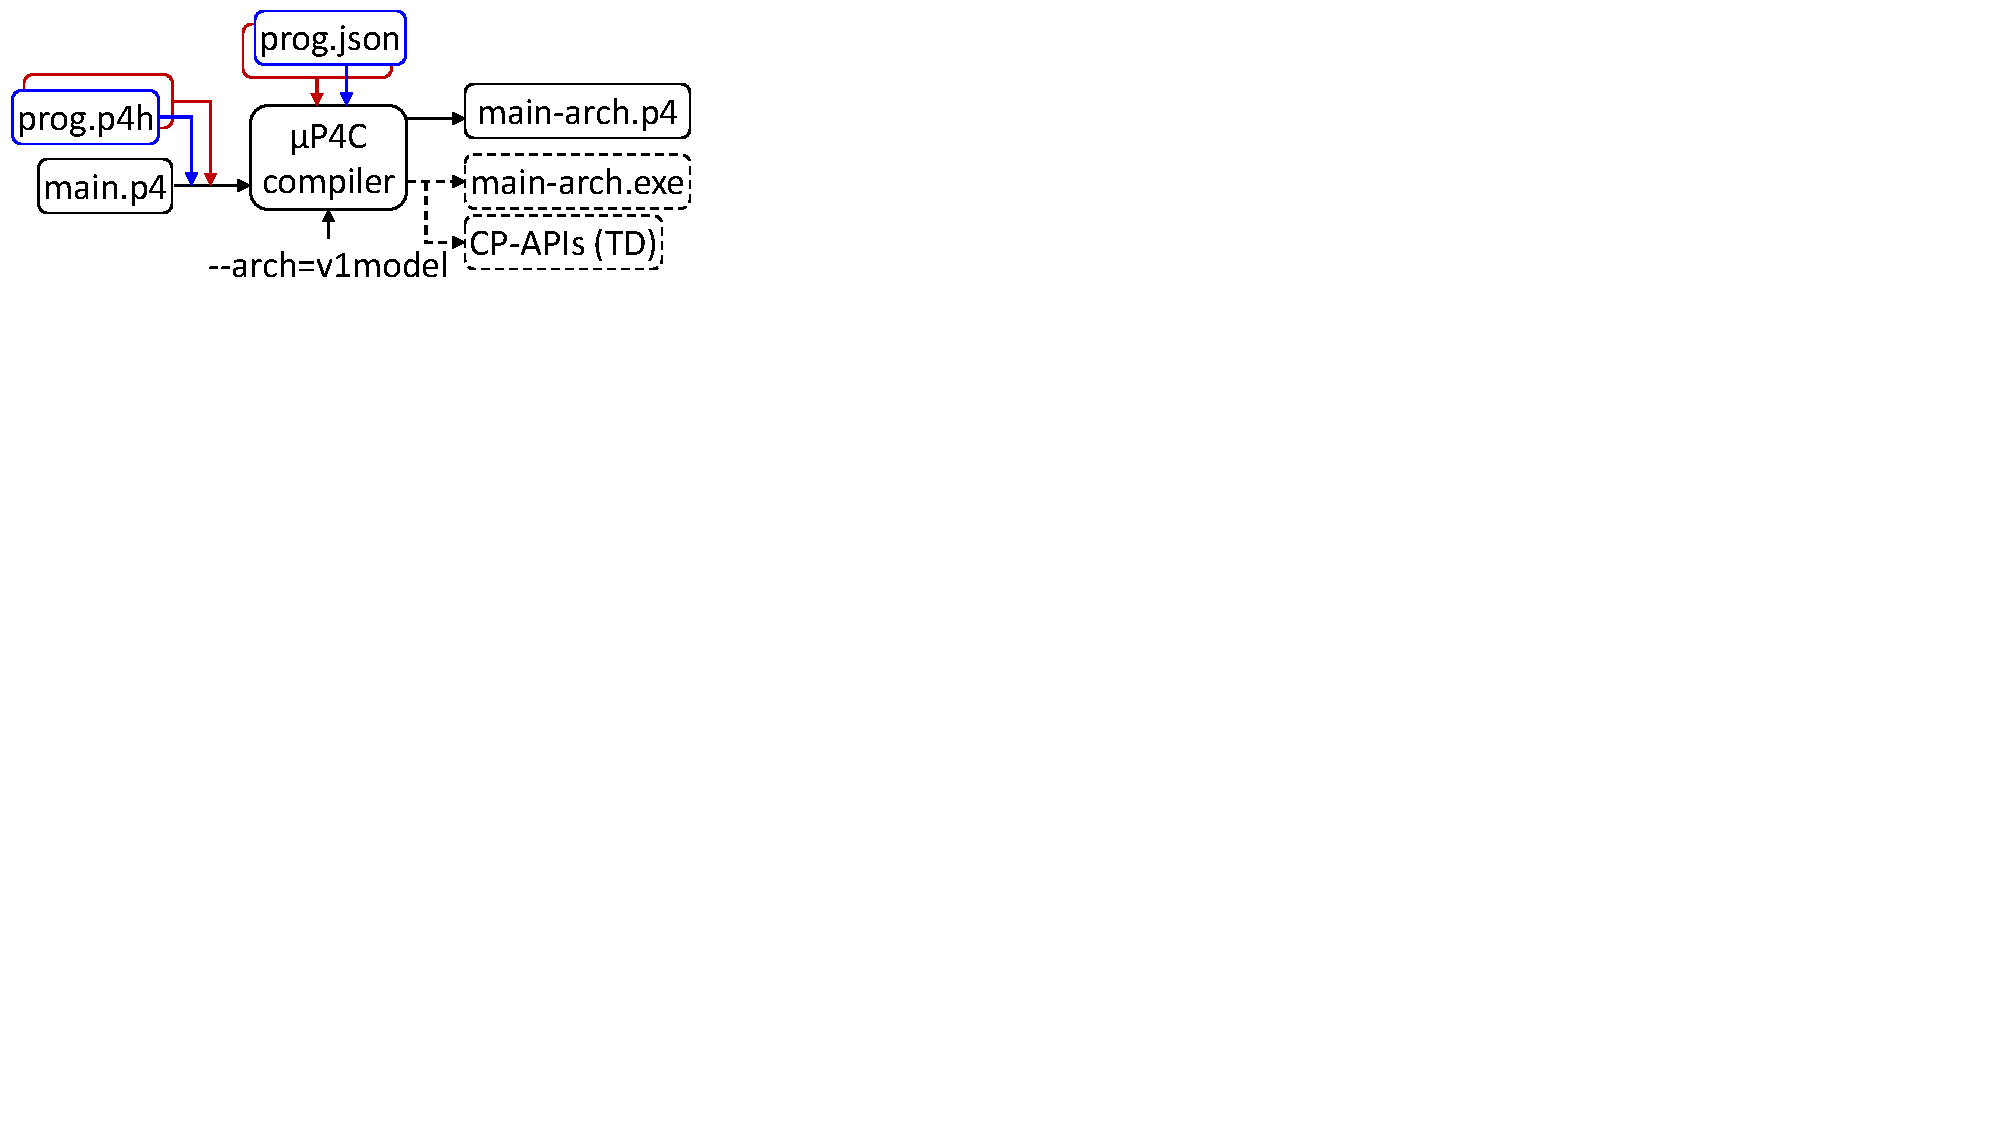
\includegraphics[trim=0 407 628 0, clip,scale=0.55]{mp4c-compiler}
        \caption{Composition and Translation of Main Instance}
        \label{subfig:composition-translation-of-main-instance}
    \end{subfigure}
\caption{Compiling $\mu$SA programs}
\label{fig:compiling-msa-programs}
\end{figure}
